\documentclass[10pt]{article}
\usepackage[a4paper, left=1.5cm, right=1.5cm, top=3.5cm]{geometry}
\usepackage[ngerman]{babel}
\usepackage[]{graphicx}
\usepackage{enumitem}
\usepackage{multicol}
\usepackage{amssymb}
\usepackage{breqn}
\usepackage{titlesec}
\usepackage{wrapfig}
\usepackage{blindtext}
\usepackage{lipsum}
\usepackage{caption}
\usepackage{listings}
\usepackage{fancyhdr}
\usepackage{nopageno}
\usepackage{authblk}
\usepackage{amsmath} % tons of math stuff
\usepackage{mathtools} % e.g. alignment within matrix
\usepackage{bm} % provides shorthand for bold in math mode
%\usepackage{esdiff} % provides derivative commands
\usepackage[ISO]{diffcoeff}
\usepackage{xcolor}
\usepackage{csquotes} % e.g. provides \enquote
\fancyhf[]{}

% own fig. env. for multicols
\newenvironment{Figure}
  {\par\medskip\noindent\minipage{\linewidth}}
  {\endminipage\par\medskip}

\begin{titlepage}
    \title{Elektronik Praktikum -- Versuch 1: Ausbreitungen von Signalen auf Leitungen}
    \author[1]{Angelo V. Brade\thanks{s72abrad@uni-bonn.de}}
    \affil[1]{Rheinische Friedrich-Wilhelms-Universität Bonn}
    \date{\today}
\end{titlepage}

\begin{document}
\pagenumbering{gobble}
\maketitle
\newpage

\tableofcontents
\newpage

\pagenumbering{arabic}

\pagestyle{fancy}
\fancyhead[R]{\thepage}
\fancyhead[L]{\leftmark}


\begin{multicols}{2}
	\section{\large Einführung}
	In diesem Versuch wird die Funktionsweise eines Differenzierglieds, der Impuls auf Kabeln, der Leitungsabschluss und die Verzögerungszeit, sowie Klippkabel und Dämpfung untersucht.
	\section{\large Theorie}
	Allgemein lässt sich jedes Gerät in 1. Ordnung durch einen Tiefpass beschreiben. Dies lässt sich anschaulich an einem Koaxialkabel verstehen. Ein Koaxialkabel besteht aus einem innerem Draht, die sog. Seele, und einem äußeren Draht, welcher von der Seele durch ein Isolator oder ein Dielektrikum getrennt ist. Meist wird zusätzlich der Äußere Draht zusätzlich von physischen außeren Einflüssen mit z.B. Plastik abgeschirmt. Nun wird der Innere und Äußere Lieter einen Kondensator bilden und, wie bei dem Herz'schen Dipol, das Kabel insgesammt eine Spule mit null Windungen darstellen.
	So gilt
	\begin{align*}
		C & = \varepsilon_r \varepsilon_0 l \frac{2\pi}{\ln\left(R_a/R_i\right)} & L & = \mu_r \mu_0 l \frac{\ln\left(R_a/R_i\right)}{2\pi}
	\end{align*}
	mit
	\begin{align*}
		\varepsilon_0 & = 8{,}85 \cdot 10^{-12} \frac{As}{Vm} & \mu_0 & = \frac{4\pi}{10} \cdot 10^{-6} \frac{Vs}{Am} \\
	\end{align*}
	So kann jedem Leiter ein Widerstand \(R\), Kapazität \(C\), Induktivität \(L\) und Verlustleitwert \(G\) zugeordnet werden. Alle Größen werden üblicher Weise durch die Kabellänge \(l\) geteilt, sodass \(X' = X/l\) gilt.
	Nun können Leiter als eine Abfolge von Tiefpassen aufgefasst werden. Hier in Abb. \ref{fig:1.1} dargestellt. Da jeder Tiefpass eine Verzögerung hat, wird so auch der Leiter insgesammt eine Verzögerung aufweisen.
	\begin{Figure}
		\centering
		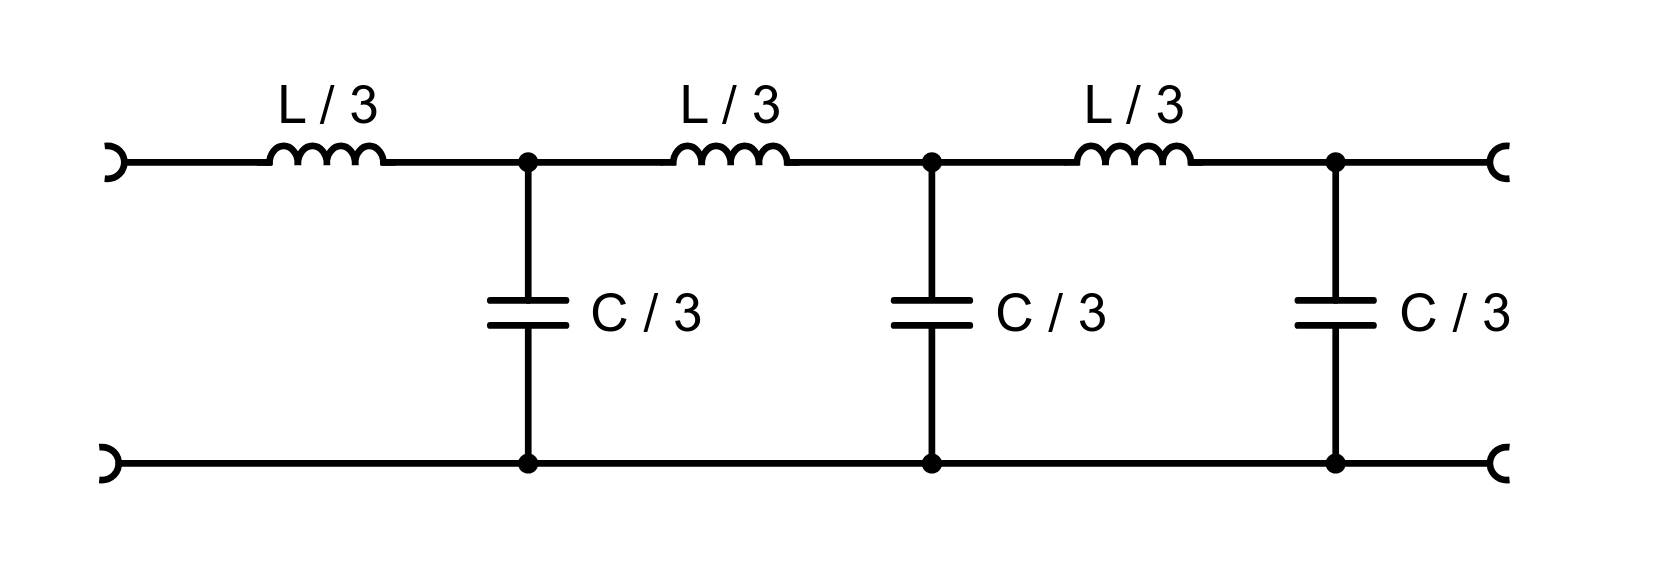
\includegraphics[width=0.9\linewidth]{Leitungsmodell.png}
		\captionof{figure}{Leitungsmodell}
		\label{fig:1.1}
	\end{Figure}
	Ferner können wir nun, wie in Abb. \ref{fig:1.2} und \ref{fig:1.3} veranschaulicht, eine Längsimpedanz \(Z := i\omega L + R\)  und eine Queradmittanz \(Y := i\omega C + G\) definieren.
	\begin{Figure}
		\centering
		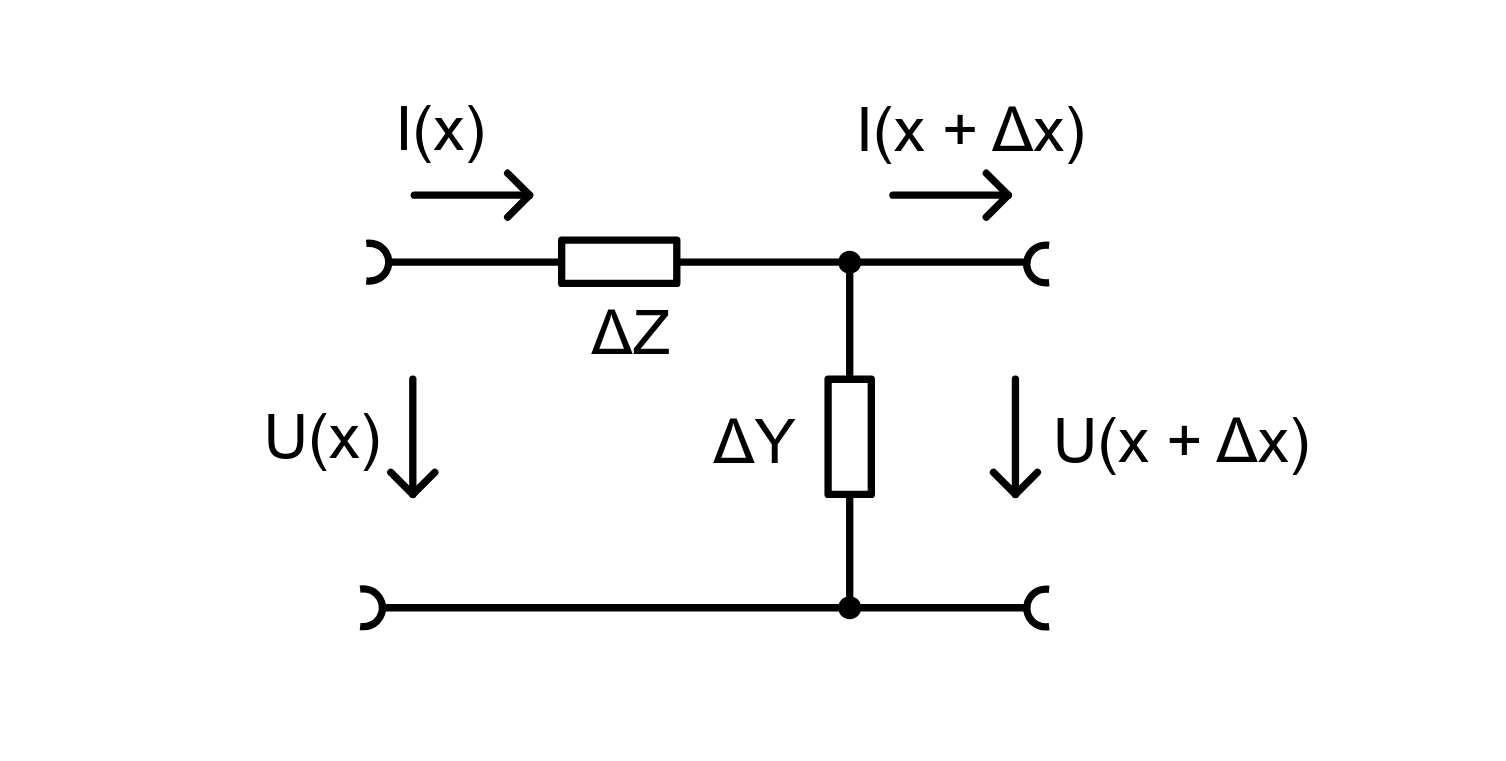
\includegraphics[width=0.9\linewidth]{Differentierglid.png}
		\captionof{figure}{Differentierglied}
		\label{fig:1.2}
	\end{Figure}
	\begin{Figure}
		\centering
		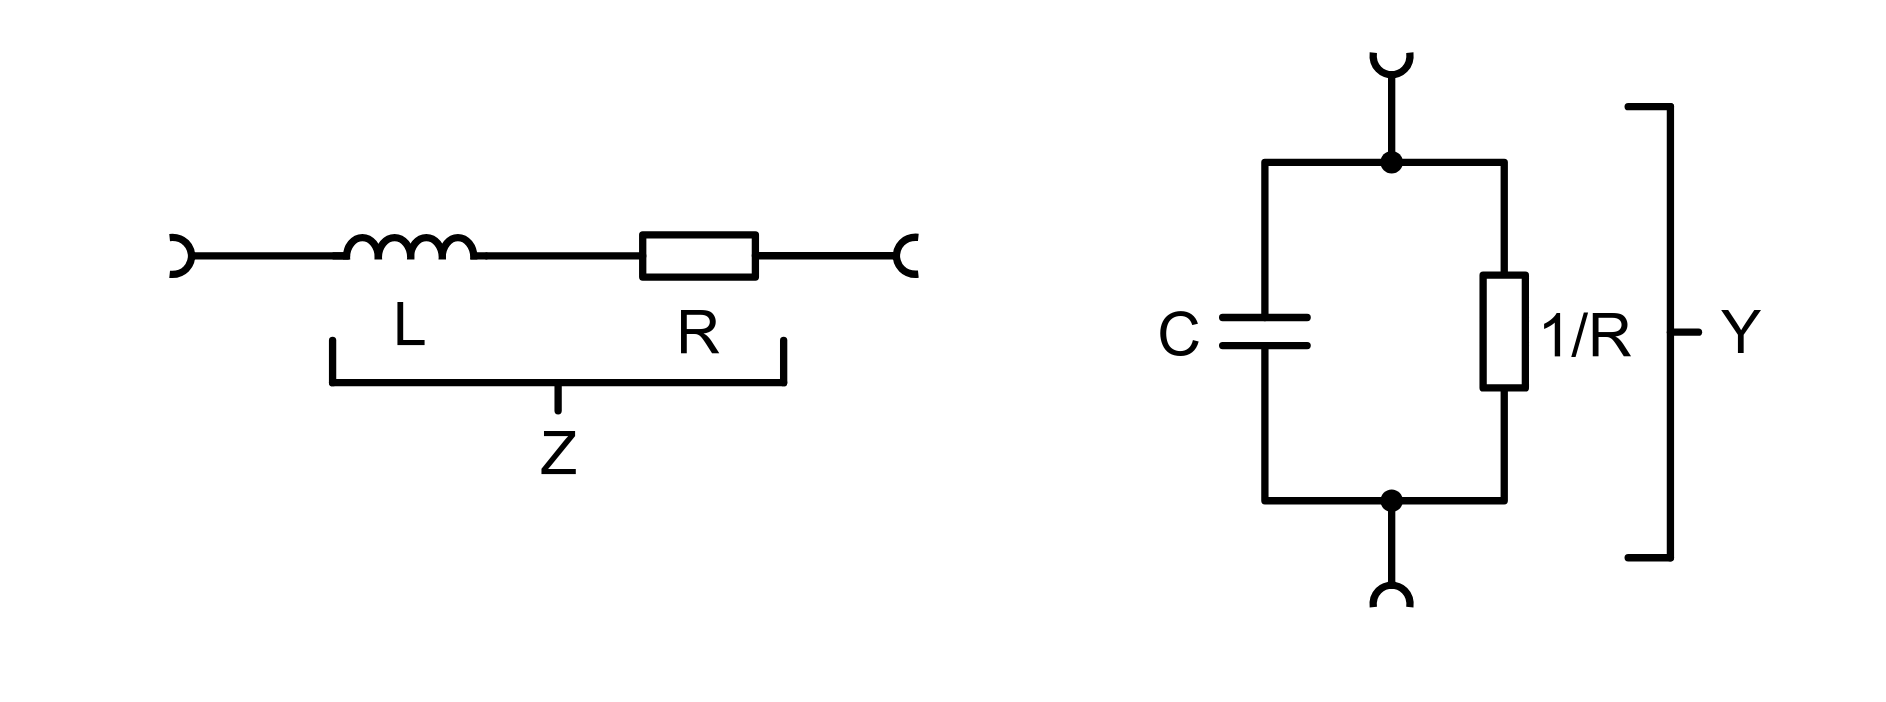
\includegraphics[width=0.9\linewidth]{Impedanzen.png}
		\captionof{figure}{Längsimpedanz Z und Queradmittanz Y}
		\label{fig:1.3}
	\end{Figure}

	Außerdem ergibt sich daraus, dass die Spannung
	\begin{align*}
		U(x, t) & = U_h(x, t) + U_r(x, t)                                                  \\
		        & = \left(U_{h0} e^{-\gamma x} + U_{r0} e^{\gamma x}\right) e^{i \omega t}
	\end{align*}
	mit
	\[
		\Upsilon^2 = Z' \cdot Y' = \left(R' + i \omega L'\right) \cdot \left(G' + i \omega C'\right)
	\]
	eine Superposition aus Hinläufiger und Rückläufiger Welle ist. Im verlustfreien Fall genügt
	\[
		\Upsilon = i \omega \sqrt{L'C'} = i \beta.
	\]
	Somit erhalten wir für die Phasen und Gruppengeschwindigkeit
	\[
    v_{\text{ph}}=v_{\text{gr}}=\frac{1}{\sqrt{L'C'}}=\frac{c_0}{\sqrt{\epsilon_r\mu_r}}
	\]
	und für den Wellenwiderstand
	\begin{align*}
		Z = \frac{U_h(x)}{I_h(x)} =\sqrt{\frac{L'}{C'}}=\sqrt{\frac{\mu_r \mu_0}{\varepsilon_r \varepsilon_0}} \cdot \frac{\ln\left(R_a/R_i\right)}{2\pi}
,
	\end{align*}
	sollten wir weiterhin den verlustfreien Fall haben.
	Nun kann an dem Kabelende, einer Glanzfläche, eine rücklaufende Welle entstehen, wenn die einlaufende Welle nicht vollständig Absorbiert wird. Die richtige Leitungsanpassung ist dann gewährleistet, sobald der Abschlusswiderstand
	\begin{align*}
		R_A & = Z\cdot\frac{1+r}{1-r} & \text{mit } r & =\frac{U_{rl}}{U_{hl}} = \frac{R_A-Z}{R_A+Z}
	\end{align*}
	dem Wellenwiderstand entspricht. Hier ist \(r:=\) Reflexionsfaktor und er müsste 0 entsprechen. So lassen sich das Stehwellenverhältnis
	\[
		s = \frac{1 + |r|}{1-|r|}
	\]
	und den Anpassungsfaktor
	\[
		m = \frac{1}{s}
	\]
	definieren.
	Nun können drei Fälle eintreten. Es gibt einen angepassten Abschluss, d.h. \(R_A=Z\), und aus der Sicht des Kabels wird das Kabel weitergeführt und es gibt keien Reflexion: \(r=0\).

	Eine Offene Leitung bedeute, dass \(R_A=\infty\) und es somit keinen Strom gäbe. Außerdem wird die Welle reflektiert, d.h. \(r=1\) und \(U_2 = 2U_{hl}\).

	Beim Kurzschluss gibt es keinen Abschlusswiderstand \(R_A=0\) und somit eine gegenläufige Refelxion, d.h \(r=-1\) und $I_2=2I_{hl}$.

	\section{\large Voraufgaben}
	\subsection{Aufgabe A}
	Um größere Verzögerungszeiten zu erreichen, muss die Phasengeschwindigkeit sinken. Also sollte nach \[
		v_{\text{ph}}=v_{\text{gr}}=\frac{1}{\sqrt{L'C'}}
	\]die Kapazität $C'$ oder die Induktivität $L'$ erhöht werden.
	\subsection{Aufgabe B}
	Wird nun die Kapazität erhöht, so erhalten wir nach
	\[
		Z =\sqrt{\frac{L'}{C'}},
	\]
  dass der Wellenwiderstand verkleinert und mit höherer Induktivität vergrößert wird.
	\subsection{Aufgabe C}
  Der Eingangswiderstand $R_{in}$ hängt nicht von der Länge des Kabels ab, da es bei einem Abschluss keine rückläufige Welle gibt.
	\subsection{Aufgabe D}
  Mit
  \[
  Z=\sqrt{\frac{\mu_r \mu_0}{\varepsilon_r \varepsilon_0}} \cdot \frac{\ln\left(R_a/R_i\right)}{2\pi}
  \]
  und
  \[
    v_{\text{ph}}=\frac{c_0}{\sqrt{\epsilon_r\mu_r}}
  \]
  erhalten wir für $R_A/R_I = 2.3, \ \varepsilon_r = 1.5 $ und $\mu_r = 1.5$, $Z\approx 49.94 \ \Omega$, $v_{ph}\approx 1.93 \times 10^{8} \ \text{ms}^{-1}$ und die Verzögerung $\Delta = \frac{1}{v_{\text{ph}}} = \frac{1.5}{c_0} \approx 5.2 \times 10^{-9} \ \text{s m}^{-1} \approx 5.2 \ \text{ns m}^{-1}$.



\end{multicols}

\end{document}
